%%%%%%%%%%%%%%%%%%%%%%%%%%%%%%%%%%%%%%%%%%%
\subsection{Polarization of EM Waves}
%%%%%%%%%%%%%%%%%%%%%%%%%%%%%%%%%%%%%%%%%%%
The polarization of EM waves is determined, for monochromatic frequencies, by the relative intensity and phase of their respective $x$ and $y$ components.  These relationships can be viewed as the path traced by the tip of the electric field vector when looking in the direction of illumination.  Common sources of illumination are lasers, light emitting diodes, halogen lamps, the sun, etc.

In its most general form, the polarization is referred to as being elliptical, and its $x$ and $y$ amplitudes, and phase delay can be described in the form of the polarization ellipse.

It has been shown that the form of the polarization ellipse can be derived from the solution to the plane wave equation for the electromagnetic wave.  Using the relationships defined in the previous section and defining,
%
\begin{align}
    \tau=\omega t-kz+\delta_x
\end{align}
%
We can then define the $x$ and $y$ component of the wave as
%
\begin{align}
	E_x (t)=E_{0x} cos(\tau)\\
	E_y (t)=E_{0y} cos(\tau+\delta )
\end{align}
%
Dividing each equation by its intensity results in
%
\begin{align}
    \frac{E_x (t)}{E_{0x}} =cos(\tau) \\
    \frac{E_y (t)}{E_{0y}} =cos(\tau+\delta )
\end{align}
%
The $y$ component is then separated using known trigonometric identities and equation
%
\begin{align}
\frac{E_y (t)}{E_{0y}} =  (cos(\tau) cos(\delta)-sin(\tau)sin(\delta))
\end{align}
%
Again using known trigonometric identities
%
\begin{align}
    \frac{E_y (t)}{E_{0y}} = \frac{E_x (t)}{E_{0x}}   cos(\delta)-\sqrt{1-\frac{E_x (t)^2}{E_{0x}^2} } sin(\delta)
\end{align}
%
Rearranging and squaring both sides results in
%
\begin{align}
    (\frac{E_x (t)}{E_{0x}}   cos(\delta)-\frac{E_y (t)}{E_{0y}} )^2=(\sqrt{1-\frac{E_x (t)^2}{E_{0x}^2} } sin(\delta))^2
\end{align}
%
The factorization of this equation can be rearranged into the standard form of an ellipse such that
%
\begin{align}
    \frac{E_x (t)^2}{E_{0x}^2} +\frac{E_y (t)^2}{E_{0y}^2} -2 \frac{E_x E_y}{E_{0x} E_{0y} } cos(\delta)=sin^2 (\delta)
\end{align}
%
And is graphed as seen in Figure 2.2.
%
\begin{figure}
    \begin{center}
        \makebox[\textwidth]{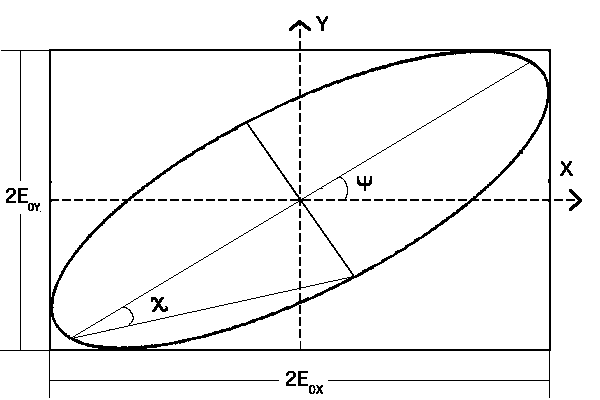
\includegraphics[scale=0.5]{/Sources/Background/Nature_of_Light/polarization-ellipse-binary-v2.png}}
    \end{center}
    \caption{Polarization Ellipse}
    \label{fig:polarization}
\end{figure}
%

Due to the restraints of modern optical sensors, it is not possible to directly measure the polarization ellipse, for a light beam, at any instant in time.  Taking the time average of the ellipse results in quantities that can measured by detectors in order to quantify the polarization state of an EM wave.  It is therefore necessary to derive parameters from the ellipse that can be measured.
Starting from the equation for the polarization ellipse, taking the time average of the E field results in
%
\begin{align}
    \frac{E_x (t)^2}{E_{0x}^2} + \frac{E_y (t)^2}{E_{0y}^2} - \frac{2 E_x (t) E_y (t)}{E_{0x} E_{0y} } cos(\delta)=sin^2 (\delta)
\end{align}
%
the time averages are calculated as
%
\begin{align}
    <E_x (t)^2> = lim_{T \rightarrow \infty} \int_{0}^{2\pi} E_{0x} cos(\tau)  d\tau=\frac{1}{2} E_{0x}^2
\end{align}
%
and similarly
%
\begin{align}
    <E_y (t)^2>  = \frac{1}{2} E_{0y}^2 \\
	<E_x (t) E_y (t)>  =  \frac{1}{2} E_{0x} E_{0y} cos(\delta)
\end{align}
%
substitution into equation and completing the square results in
%
\begin{align}
    (E_{0x}^2+E_{0x}^2 )^2-(E_{0x}^2-E_{0x}^2 )^2-(2E_{0x}^2 E_{0x}^2  cos(\delta) )^2=(2E_{0x} E_{0y}  sin(\delta))^2
\end{align}
%
The terms of this equation represent the polarization state of a wave in relation to the x and y intensities and relative phase delay between the two components.
These quantities are known as the Stokes parameters and describe the state of polarization and are often represented as a vector,
%
\begin{align}
    \vec{S} =
    \begin{bmatrix}
        S_0 \\
        S_1 \\
        S_2 \\
        S_3
    \end{bmatrix}
    =
    \begin{bmatrix}
        E_{0x}^2+E_{0y}^2 \\
        E_{0x}^2-E_{0y}^2 \\
        2E_{0x}^2 E_{0y}^2 cos(\delta) \\
        2E_{0x} E_{0y}  sin(\delta)
    \end{bmatrix}
\end{align}
%
The degree of polarization for an EM wave is the magnitude of the Stokes vector such that
%
\begin{align}
    \alpha =DOP=  \frac{\sqrt{S_1^2+S_2^2+S_3^2 }}{S_0}
\end{align}
%
and ranges from 0 for unpolarized light, to 1 for completely polarized light.  It is possible to show the polarized and unpolarized intensities as individual components
summed together as
%
\begin{align}
    S=S_P+S_U=
    \begin{bmatrix}
        S_0 \\
        S_1 \\
        S_2 \\
        S_3
    \end{bmatrix}
    +(1-DOP)
    \begin{bmatrix}
        1 \\
        0 \\
        0 \\
        0
    \end{bmatrix}
\end{align}
%
The degree of polarization for the linear (DOLP) and circular polarization (DOCP) can specifically be quantified as
%
\begin{align}
    DOLP=  \frac{\sqrt{S_1^2+S_2^2 }}{S_0} \\
    DOCP=  \frac{S_3}{S_0}
\end{align}
%
Note the unpolarized light is represented as
%
\begin{align}
    S=
    \begin{bmatrix}
        S_0 \\
        S_1 \\
        S_2 \\
        S_3
    \end{bmatrix}
    =
    \begin{bmatrix}
        1 \\
        0 \\
        0 \\
        0
    \end{bmatrix}
\end{align}
%
The Stokes parameters can be graphed on a unit sphere, known as the Poincare sphere.  The sphere plots the radial coordinates describing ellipticity and eccentricy of the polarization ellipse as angles of
%
\begin{align}
    Ellipicity = \frac{S_3}{S_0+\sqrt{S_1^2+S_2^2 }}
\end{align}
\begin{align}
    Eccentricity= \sqrt{1-Ellipticity^2}
\end{align}
%
The ellipticity of the polarization ellipse varies from 0, for linearly polarized light, to 1 for purely circular polarization \cite{chipman}.
%
For	graphical representation, Stokes vectors can be plotted on a 3-dimensional sphere known as the Poincare sphere. The sphere is only capable of showing the polarized portion of the EM wave.  Prior to normalization, if the EM wave is not fully polarized, the intensity of the polarized beam must be normalized in relation to the total beam intensity.
%
\begin{figure}[!htb]
    \begin{center}
        \makebox[\textwidth]{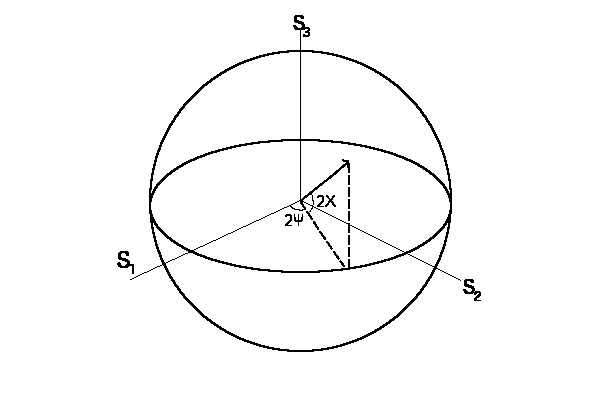
\includegraphics[scale=0.6]{/Sources/Background/Nature_of_Light/POINCARE-binary.png}}
    \end{center}
    \caption{Poincare Sphere}
    \label{fig:polarization}
\end{figure}
%
The zenith angle of the polarization ellipse, represented in Figure 2.3 as $2\chi$ is found to be related to the parameters of the polarization ellipse by
%
\begin{align}
    sin2\chi = \frac{2E_{0x}2E_{0y}sin\delta}{E_{0x}^2+E_{0y}^2}\qquad -\pi / 4 \leq \chi \leq \pi / 4
\end{align}
%
The azimuth angle $2\psi$ is defined in relation to the parameters of the polarization ellipse as
%
\begin{align}
    tan2\psi = \frac{2E_{0x}2E_{0y}cos\delta}{E_{0x}^2-E_{0y}^2}\qquad 0 \leq \psi \leq \pi
\end{align}
%
For a given state of the polarization ellipse, the angles for plotting the corresponding polarization state on the Poincare sphere can be found using these equations\cite{spieellipse}.
